\documentclass{standalone}
\usepackage{tikz}
\begin{document}
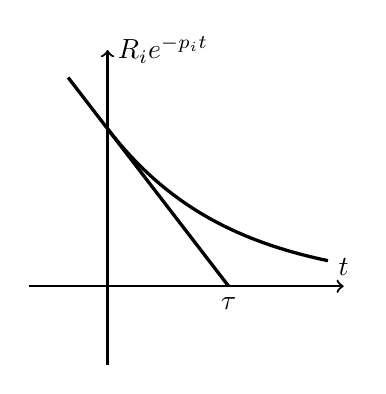
\begin{tikzpicture}[scale=2]
    \draw[->,thick](-0.5,0)--(1.5,0)node[above]{$t$};
    \draw[->,thick](0,-0.5)--(0,1.5)node[right]{$R_ie^{-p_it}$};

    \draw[-,very thick]plot[smooth, domain=0:1.4](\x,{e^(-1.3*\x)});
    \draw[-,very thick]plot[smooth, domain=-0.25:0](\x,{-1.3*\x+1});
    \draw[-,very thick](0,1)--(0.769,0)node[below]{$\tau$};
\end{tikzpicture}
\end{document}